\documentclass[11pt]{article}
\usepackage[utf8]{inputenc}
\usepackage{amsmath}
\usepackage{eurosym}
\usepackage{graphicx}
\usepackage{libertine}
\usepackage{microtype}
\usepackage{titlesec}
\titlespacing\section{0pt}{12pt plus 4pt minus 2pt}{0pt plus 2pt minus 2pt}
\titlespacing\subsection{0pt}{12pt plus 4pt minus 2pt}{0pt plus 2pt minus 2pt}
\titlespacing\subsubsection{0pt}{12pt plus 4pt minus 2pt}{0pt plus 2pt minus 2pt}
\usepackage{enumitem}
\setlist{nosep}
\usepackage[left=2.5cm,right=2.5cm,top=1.75cm,bottom=1.75cm,a4paper]{geometry}
\usepackage[hidelinks,colorlinks]{hyperref}

\let\oldFootnote\footnote
\newcommand\nextToken\relax

\renewcommand\footnote[1]{%
    \oldFootnote{#1}\futurelet\nextToken\isFootnote}

\newcommand\isFootnote{%
    \ifx\footnote\nextToken\textsuperscript{,}\fi}

\makeatletter
\def\@maketitle{%
  \newpage
  \begin{center}%
  \let \footnote \thanks
    {\LARGE\bfseries \@title \par}%
    \vskip 1em%
    {\large \@date}%
  \end{center}%
  \par
  \vskip 1em}
\makeatother	
	

\title{For Overlay Journals in Mechanics}
%\author{Vincent Acary [Inria Grenoble] and Mathias Legrand [McGill University]}
%\date{}
\begin{document}
\maketitle
\noindent The purpose of this letter is to raise awareness about \emph{Overlay Journal} publications among the scholarly communities in Mechanics. Relevant hyperlinks are given as footnotes.
\section*{Problem}
How is all this possible? Tomorrow, researchers will have to pay in order to publish! The Gold Open Access model with Article Processing Charge (APC) seems to expand rapidly in our communities. This publication process uses a business model based on individual articles for which their authors pay fees for publication.\footnote{\href{https://en.wikipedia.org/wiki/Article_processing_charge}{Definition of APC on Wikipedia}}

\section*{Public finances}
This model will have dramatic consequences on universities' and research institutes' budgets, and more generally on public finances. For instance in France, CNRS currently spends about M\EUR{15}/year in library resources, amount that is expected to reach M\EUR{95}/year in case Gold Access with APC becomes the preferred avenue for publishing.\footnote{\href{http://www.cnrs.fr/dist/z-outils/documents/Distinfo2/DISTetude_4.pdf}{DIST Etude 2015 assuming that all CNRS authors will pay for their contributions.}} Similar numbers are provided by McGill's library concerning the subscription to journals and electronic resources.\footnote{\href{http://www.mcgill.ca/library/files/library/mcgill_library_and_archives_-_annual_report_2016_0.pdf}{2016 Annual Report, page 13}} Moreover, the H2020 program promotes Open Access in the general sense (with or without APC) that could have an harmful side-effect in case no alternative to APC is available. The fact that APC are eligible expenses to be listed in proposals of H2020 is a consequence of this ambiguity.
Some of you might think that overall APC count as a minor fraction of research expenses. This is probably true. However, financial savings at the scale of a country are not negligible if a publication process free of charges for both authors and readers, in agreement with the Diamond Open Access Policy,\footnote{\href{https://en.wikipedia.org/wiki/Open_access_journal}{Definition of Diamond Access Policy}} is implemented.

\section*{Open Access, sustainable research and Overlay Journals}
As our colleagues in Mathematics, Computer Science and Human Sciences have already understood,\footnote{\href{https://www.cimpa.info/en/node/62}{List of Mathematical Journals that apply a Diamond Open Access policy}}\footnote{\href{https://www.episciences.org/page/journals}{épisciences.org Overlay Journals}} Overlay Journals (also called \emph{Epijournals}) are the way to go! Overlay journals are purely open access electronic journals solely fed by articles that are deposited on Open Archives (arXiv, HAL, engrXiv...) and not already published elsewhere. The review procedure, undertaken by the editorial team of the Overlay Journal together with designated reviewers, is of high quality\footnote{\href{http://discreteanalysisjournal.com/articles and its announcement by Nature https://www.nature.com/news/leading-mathematician-launches-arxiv-overlay-journal-1.18351}{Discussion on the Discrete Analysis Overlay Journal in Mathematics}}. This virtuous framework induces a minimal cost to society and taxpayers while publications (and possibly attendant data) are always openly accessible on the long run with permanent url links. Technical challenges are minimal since appropriate platforms already exist. As an example, the Episciences initiative\footnote{\href{https://www.episciences.org/?lang=en}{épisciences.org Website}} provides technical support for peer-reviewing activities which are supervised by editorial boards. To summarize, Overlay Journals add value to Open Archives by assigning a scientific caution to the accepted papers. 
Overlay Journals ensure the same Diamond OA but at much smaller expenses of public funds and are open to everyone who conducts a high quality research irrespective of research funds of the individual.
Other benefits of Diamond Open Access are summarized in Figure~\ref{fig:OA}.
\begin{figure}[ht]\centering%
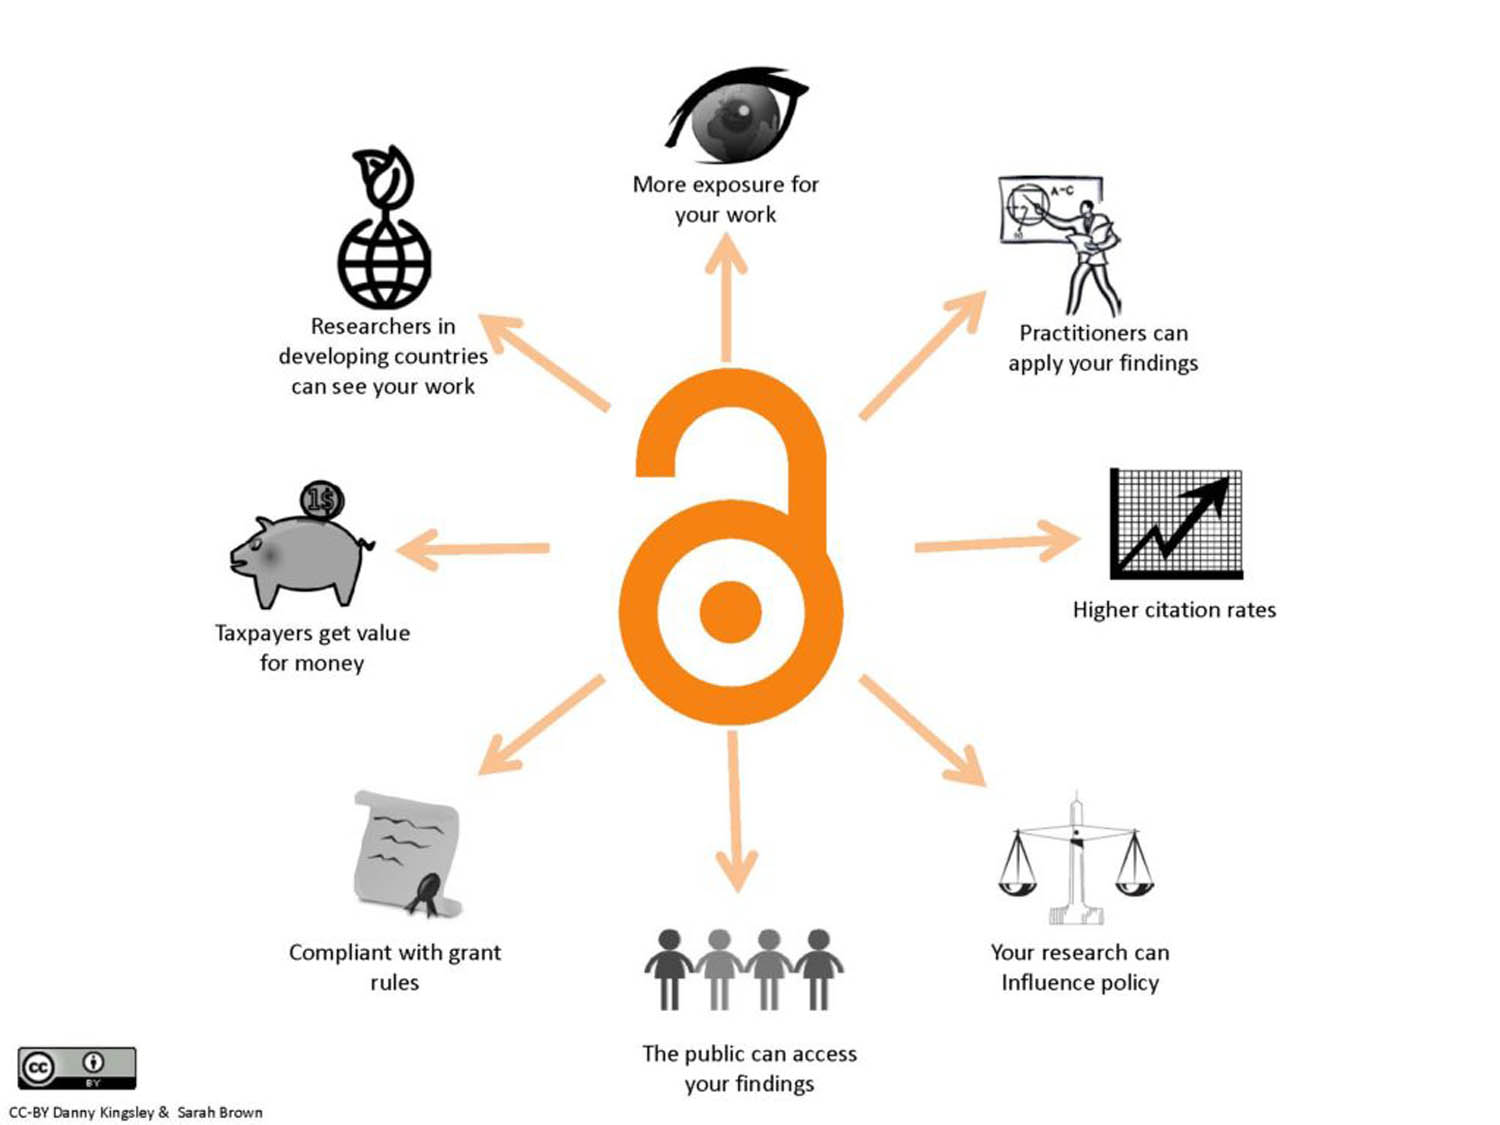
\includegraphics[width=14cm]{OA.jpg}\caption{Benefits of Diamond Open Access}\label{fig:OA}
\end{figure}

\section*{And the Mechanics community?}
It is now critical that the mechanics community thinks about a full open access model to publish the outcomes of research, and more specifically about the creation of Overlay Journals in various subfields of Mechanics. Lately, this question generated a strong interest as it is witnessed by the fruitful discussion\footnote{\href{https://www.loomio.org/invitations/aa0a97be9a80ba509623}{Loomio discussion on Overly Journals in Mechanics}} on Loomio, an online tool increasing transparency and inclusion to reach decisions.

\section*{Next steps and questions to the Scholarly Society}
For the success of this initiative the involvement of Scholarly Socities is of paramount importance. It would greatly simplify the creation of Overlay Journals and blow a wind of change able to completely redraw the arcane of publishing. As a first step, an international editorial board should now be created and we would welcome a formal reply to the questions posed below. This Overlay Journal item could be discussed during your next steering committee.
\begin{itemize}
\item Would the Society position itself as a proponent of alternative publication processes based on Overlay Journals? 
\item Could the Society suggest a list of members to the editorial board and/or scientific committee for the Overlay Journal? 
\item Could the Society encourage submissions of papers submitted to International Conferences and Workshops that it sponsors? 
\item Would the Society be able to support this initiative of creating an Overlay Journal in Mechanics and how?
\end{itemize}
It is also worth noting that the present letter has been sent to the following Scholarly Societies: IUTAM, IACM, EUROMECH, EASD, MECAMAT, AFM, CSMA, ECCOMAS, and CNFM. All the answers will be made publicly available at the address: {\small\text{\url{https://epijournalinmechanics.github.io}}}.\\[5pt]

On behalf of the Loomio members supporting the creation of Overlay Journals in Mechanics, \\[10pt]
Vincent Acary, INRIA, France\\
Mathias Legrand, McGill University, Canada\\
Maurine Montagnat, CNRS, France\\
Vladislav Yastrebov, CNRS, MINES ParisTech, France
\end{document}

%%% Local Variables:
%%% mode: latex
%%% TeX-master: t
%%% End:
